\documentclass[]{../../../../tex/classes/homework}
\usepackage{../../../../tex/packages/hebrewSupport}
\usepackage{../../../../tex/packages/mathShortcuts}
\usepackage{../../../../tex/packages/theoremsSupport}

\usepackage{float}


\definecolor{yell}{RGB}{204, 153, 0}
\definecolor{gr}{RGB}  {0, 180, 20}
\newcommand\DC{$\vn$}
\newcommand\karno[1]{\begin{center}
		\begin{minipage}{\linewidth}
			\centering
			\includegraphics[width=0.4\linewidth]{images/#1}
		\end{minipage}
\end{center}}
\newcommand\logisim[1]{\begin{figure}[H]
		\centering
		\includegraphics[width=300pt]{images/#1}
\end{figure}}

\author{שחר פרץ}
\title{מבנה מחשבים $\sim$ \textit{תרגיל בית 1}}
\begin{document}
	\maketitle
	\section{}
	\begin{enumerate}[(A)]
		\item נוכיח ש־$xy + x'z + yz = xy + x'z$. \begin{proof}
			\begin{align*}
				xy + x'z + yz &= xy + x'z + yz(x + x') \\
				&= xy + x'z + yzx + yzx' \\
				&= x(y + yz) + x'(z + zy) \\
				&= xy\underbrace{(1 + z)}_1 + x'z\underbrace{(1 + y)}_1 \\
				&= xy + x'z
			\end{align*}
			כנדרש. 
		\end{proof}
		\item נתון $x'y + xy' = z$. נוכיח $xz' + x'z = y$. \begin{proof}
			מדה מורגן + פתיחת סוגריים $z' = (x'y + xy')' = (x + y')(y + x') = xy + yy' + xx' + x'y' = xy + x'y'$. לכן: 
			\[ xz' + x'z = x(xy + x'y') + x'(x'y + xy') = xxy + \cancel{xx'y} + x'x'y + \cancel{x'xy'} = xy + x'y  = y \]
			כנדרש. 
		\end{proof}
		\item רשות
	\end{enumerate}
	
	\section{}
	נממש שער \en{OR} \ בעל 4 כניסות ויציאה אחת (הפונקציה $F(x, y, z, w) = x + y + z + w$). 
	\begin{enumerate}
		\item בעזרת שערי \en{NOR $3 \to 1$}\ ושערי \en{NOT}: 
		\logisim{q2a}
		\item בעזרת שערי \en{NOR}\  ו־\en{NAND}: 
		\logisim{q2b}
	\end{enumerate}
	
	\section{}
	\begin{enumerate}[(A)]
		\item נבטא את הפונקציה $F(x, y, z) = x + y + \bar xz + y\bar z$ באמצעות שערים ספציפיים בלי לפשט אותה כלל (הערה: ליתר בטחון לא פישטתי בשום צורה, גם אם במימוש שלי יש שני NOT־ים אחד אחרי השני)
		\begin{enumerate}[i.]
			\item בעזרת שערי \en{OR}, \en{AND}\ ו־\en{NOT}\ בלבד: 
			\logisim{q3a}
			\item בעזרת שערי \en{AND}\ ו־\en{NOT}\ בלבד: 
			\logisim{q3b}
			\item בעזרת שערי \en{NAND}\ בלבד: 
			\logisim{q3c}
			\item בעזרת שערי \en{OR}\ ו־\en{NOT}\ בלבד: 
			\logisim{q3d}
		\end{enumerate}
		\item נרשום מפת קרנו בעבור בפונקציה מסעיף 1: 
		\begin{figure}[h]
			\centering
			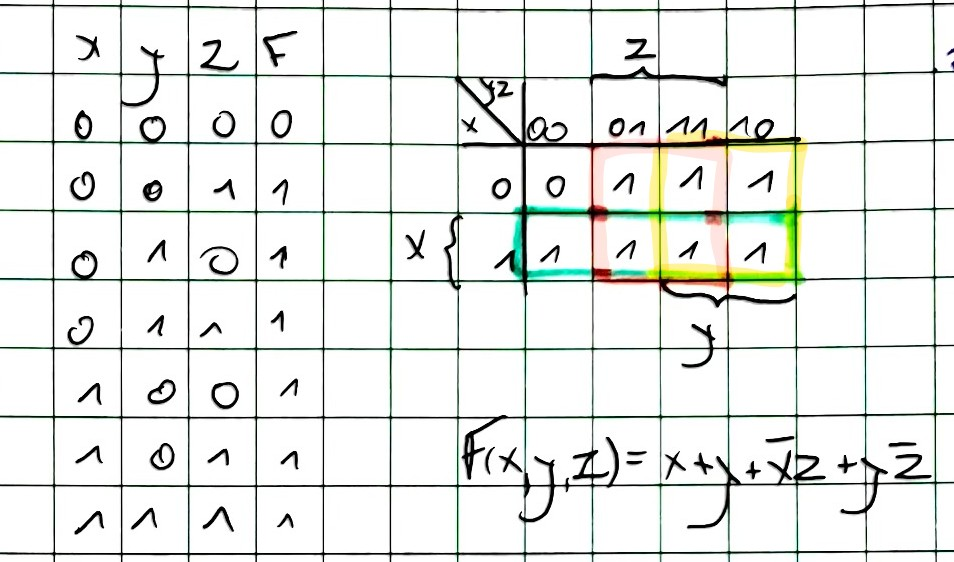
\includegraphics[width=0.4\linewidth]{images/q2_1}
		\end{figure}
		
		נבחין שהפונקציה שקיבלנו היא $F(x, y, z) = {\color{red}z} + {\color{cyan}x} + {\color{yell}y}$. לכן מימושה יהיה: 
		\begin{figure}[H]
			\centering
			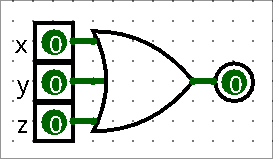
\includegraphics[width=150pt]{images/q3last}
		\end{figure}
	\end{enumerate}
	
	\section{}
	נתונה מפת קרנו: 
	\begin{enumerate}[(A)]
		\item נרשום את ה־SoP המינימלי עבור המפה:
		
		נבחין ש־: 
		\begin{figure}[h]
			\centering
			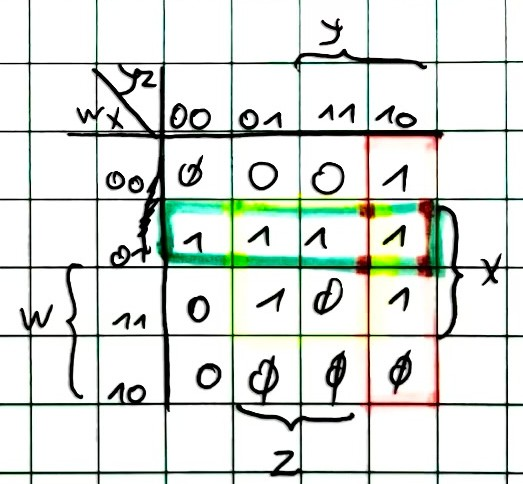
\includegraphics[width=0.2\linewidth]{images/q4_A1}
		\end{figure}
		\[ F_1(x, y, z, w) = {\color{yell}xz} + {\color{red}{yz'}} + {\color{cyan}w'x} \]
		
		אשר ליחידות הביטוי – אם קיים (עד כדי don't cares) איזשהו קיבוץ של ה־1־ים חוקי (ומינימלי) אחר למפת הקרנו, אזי הביטוי איננו יחיד. אכן נוכל למצוא קיבוץ כזה: 
		\begin{figure}[h]
			\centering
			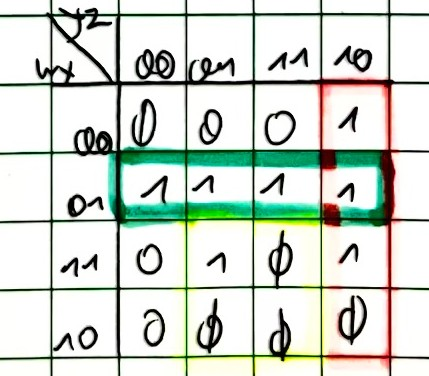
\includegraphics[width=0.2\linewidth]{images/q4_A2}
		\end{figure}
		
		\[ F_2(x, y, z, w) = {\color{yell}zw} + {\color{red}{yz'}} + {\color{cyan}w'x} \]
		
		\item נמצא את ה־PoS המינימלי, נקבץ את האפסים בטבלה במקום, נמצא את ה־SoP של הפונקציה המשלימה, ואז נשתמש בכללי דה־מורגן. 
		
		נבחין ש־: 
		\begin{figure}[h]
			\centering
			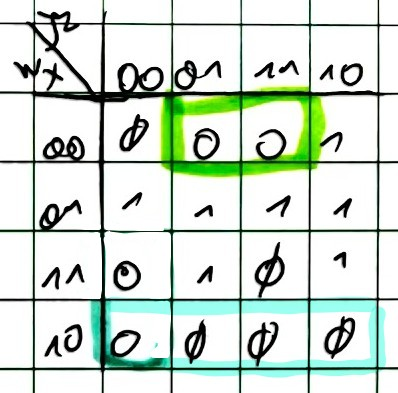
\includegraphics[width=0.2\linewidth]{images/q4_B}
		\end{figure}
		\[ \ol f = {\color{gr}zw'x'} + {\color{cyan}wx'} \]
		ולכן ה־PoS המינימלי הוא: 
		\[ f = (\ol f)' = (zw'x' + wx')' = \bm{(z' + w + x) \cdot (w' + x)} \]
	\end{enumerate}
	
	\section{}
	\textbf{הערה: }השתמשתי בקידוד של ארבעת הסיביות לפי {yzwx} במקום {wxyz} מטעמי נוחות. זה כמובן לא משפיע על אופן הפתרון. 
	\begin{enumerate}
		\item נבנה טבלת אמת בעבור כל יציאה במקטעי ההארה. 
		\begin{multicols}{3}
			\begin{enumerate}
				\item \begin{center}
					\begin{tabular}{ c c c c c|c }
						\en{No.} & y & z & w & x & F \\
						\hline
						   & 0 & 0 & 0 & 0 & \DC \\ 
						   & 0 & 0 & 0 & 1 & \DC \\ 
						   & 0 & 0 & 1 & 0 & \DC \\ 
						$0$& 0 & 0 & 1 & 1 & 1 \\ 
						$1$& 0 & 1 & 0 & 0 & 0 \\ 
						$2$& 0 & 1 & 0 & 1 & 1 \\ 
						$3$& 0 & 1 & 1 & 0 & 1 \\ 
						$4$& 0 & 1 & 1 & 1 & 0 \\ 
						$5$& 1 & 0 & 0 & 0 & 1 \\ 
						$6$& 1 & 0 & 0 & 1 & 1 \\ 
						$7$& 1 & 0 & 1 & 0 & 1 \\ 
						$8$& 1 & 0 & 1 & 1 & 1 \\
						$9$& 1 & 1 & 0 & 0 & 1 \\ 
						   & 1 & 1 & 0 & 1 & \DC \\ 
						   & 1 & 1 & 1 & 0 & \DC \\ 
						   & 1 & 1 & 1 & 1 & \DC
					\end{tabular}
				\end{center}
				\item \begin{center}
					\begin{tabular}{ c c c c c|c }
						\en{No.} & y & z & w & x & F \\
						\hline
						   & 0 & 0 & 0 & 0 & \DC \\ 
						   & 0 & 0 & 0 & 1 & \DC \\ 
						   & 0 & 0 & 1 & 0 & \DC \\ 
						$0$& 0 & 0 & 1 & 1 & 1 \\ 
						$1$& 0 & 1 & 0 & 0 & 1 \\ 
						$2$& 0 & 1 & 0 & 1 & 1 \\ 
						$3$& 0 & 1 & 1 & 0 & 1 \\ 
						$4$& 0 & 1 & 1 & 1 & 1 \\ 
						$5$& 1 & 0 & 0 & 0 & 0 \\ 
						$6$& 1 & 0 & 0 & 1 & 0 \\ 
						$7$& 1 & 0 & 1 & 0 & 1 \\ 
						$8$& 1 & 0 & 1 & 1 & 1 \\
						$9$& 1 & 1 & 0 & 0 & 1 \\ 
						   & 1 & 1 & 0 & 1 & \DC \\ 
						   & 1 & 1 & 1 & 0 & \DC \\ 
						   & 1 & 1 & 1 & 1 & \DC
					\end{tabular}
				\end{center}
				\item \begin{center}
					\begin{tabular}{ c c c c c|c }
						\en{No.} & y & z & w & x & F \\
						\hline
						   & 0 & 0 & 0 & 0 & \DC \\ 
						   & 0 & 0 & 0 & 1 & \DC \\ 
						   & 0 & 0 & 1 & 0 & \DC \\ 
						$0$& 0 & 0 & 1 & 1 & 1 \\ 
						$1$& 0 & 1 & 0 & 0 & 1 \\ 
						$2$& 0 & 1 & 0 & 1 & 0 \\ 
						$3$& 0 & 1 & 1 & 0 & 1 \\ 
						$4$& 0 & 1 & 1 & 1 & 1 \\ 
						$5$& 1 & 0 & 0 & 0 & 1 \\ 
						$6$& 1 & 0 & 0 & 1 & 1 \\ 
						$7$& 1 & 0 & 1 & 0 & 1 \\ 
						$8$& 1 & 0 & 1 & 1 & 1 \\
						$9$& 1 & 1 & 0 & 0 & 1 \\ 
						   & 1 & 1 & 0 & 1 & \DC \\ 
						   & 1 & 1 & 1 & 0 & \DC \\ 
						   & 1 & 1 & 1 & 1 & \DC
					\end{tabular}
				\end{center}
				\item \begin{center}
					\begin{tabular}{ c c c c c|c }
						\en{No.} & y & z & w & x & F \\
						\hline
						   & 0 & 0 & 0 & 0 & \DC \\ 
						   & 0 & 0 & 0 & 1 & \DC \\ 
						   & 0 & 0 & 1 & 0 & \DC \\ 
						$0$& 0 & 0 & 1 & 1 & 1 \\ 
						$1$& 0 & 1 & 0 & 0 & 0 \\ 
						$2$& 0 & 1 & 0 & 1 & 1 \\ 
						$3$& 0 & 1 & 1 & 0 & 1 \\ 
						$4$& 0 & 1 & 1 & 1 & 0 \\ 
						$5$& 1 & 0 & 0 & 0 & 1 \\ 
						$6$& 1 & 0 & 0 & 1 & 1 \\ 
						$7$& 1 & 0 & 1 & 0 & 0 \\ 
						$8$& 1 & 0 & 1 & 1 & 1 \\
						$9$& 1 & 1 & 0 & 0 & 0 \\ 
						   & 1 & 1 & 0 & 1 & \DC \\ 
						   & 1 & 1 & 1 & 0 & \DC \\ 
						   & 1 & 1 & 1 & 1 & \DC
					\end{tabular}
				\end{center}
				\item \begin{center}
					\begin{tabular}{ c c c c c|c }
						\en{No.} & y & z & w & x & F \\
						\hline
						   & 0 & 0 & 0 & 0 & \DC \\ 
						   & 0 & 0 & 0 & 1 & \DC \\ 
						   & 0 & 0 & 1 & 0 & \DC \\ 
						$0$& 0 & 0 & 1 & 1 & 1 \\ 
						$1$& 0 & 1 & 0 & 0 & 0 \\ 
						$2$& 0 & 1 & 0 & 1 & 1 \\ 
						$3$& 0 & 1 & 1 & 0 & 0 \\ 
						$4$& 0 & 1 & 1 & 1 & 0 \\ 
						$5$& 1 & 0 & 0 & 0 & 0 \\ 
						$6$& 1 & 0 & 0 & 1 & 1 \\ 
						$7$& 1 & 0 & 1 & 0 & 0 \\ 
						$8$& 1 & 0 & 1 & 1 & 1 \\
						$9$& 1 & 1 & 0 & 0 & 0 \\ 
						   & 1 & 1 & 0 & 1 & \DC \\ 
						   & 1 & 1 & 1 & 0 & \DC \\ 
						   & 1 & 1 & 1 & 1 & \DC
					\end{tabular}
				\end{center}
				\item \begin{center}
					\begin{tabular}{ c c c c c|c }
						\en{No.} & y & z & w & x & F \\
						\hline
						   & 0 & 0 & 0 & 0 & \DC \\ 
						   & 0 & 0 & 0 & 1 & \DC \\ 
						   & 0 & 0 & 1 & 0 & \DC \\ 
						$0$& 0 & 0 & 1 & 1 & 1 \\ 
						$1$& 0 & 1 & 0 & 0 & 0 \\ 
						$2$& 0 & 1 & 0 & 1 & 0 \\ 
						$3$& 0 & 1 & 1 & 0 & 0 \\ 
						$4$& 0 & 1 & 1 & 1 & 1 \\ 
						$5$& 1 & 0 & 0 & 0 & 1 \\ 
						$6$& 1 & 0 & 0 & 1 & 1 \\ 
						$7$& 1 & 0 & 1 & 0 & 0 \\ 
						$8$& 1 & 0 & 1 & 1 & 1 \\
						$9$& 1 & 1 & 0 & 0 & 1 \\ 
						   & 1 & 1 & 0 & 1 & \DC \\ 
						   & 1 & 1 & 1 & 0 & \DC \\ 
						   & 1 & 1 & 1 & 1 & \DC
					\end{tabular}
				\end{center}
				\columnbreak
				\item \begin{center}
					\begin{tabular}{ c c c c c|c }
						\en{No.} & y & z & w & x & F \\
						\hline
						   & 0 & 0 & 0 & 0 & \DC \\ 
						   & 0 & 0 & 0 & 1 & \DC \\ 
						   & 0 & 0 & 1 & 0 & \DC \\ 
						$0$& 0 & 0 & 1 & 1 & 0 \\ 
						$1$& 0 & 1 & 0 & 0 & 0 \\ 
						$2$& 0 & 1 & 0 & 1 & 1 \\ 
						$3$& 0 & 1 & 1 & 0 & 1 \\ 
						$4$& 0 & 1 & 1 & 1 & 1 \\ 
						$5$& 1 & 0 & 0 & 0 & 1 \\ 
						$6$& 1 & 0 & 0 & 1 & 1 \\ 
						$7$& 1 & 0 & 1 & 0 & 0 \\ 
						$8$& 1 & 0 & 1 & 1 & 1 \\
						$9$& 1 & 1 & 0 & 0 & 1 \\ 
						   & 1 & 1 & 0 & 1 & \DC \\ 
						   & 1 & 1 & 1 & 0 & \DC \\ 
						   & 1 & 1 & 1 & 1 & \DC
					\end{tabular}
				\end{center}
			\end{enumerate}
		\end{multicols}
		\item נפשט בעזרת מפות קרנו את כל אחת מהיציאות לסכום מינימלי: 
		\begin{multicols}{2}
			\begin{enumerate}
				\item \hfil $F_a(x, y, z, w) = {\color{cyan}y} + {\color{yell}{xw'}} + {\color{red}z'} + {\color{gr}x'w}$
				\karno{q5_a}
				\item \hfil $F_b(x, y, z, w) = {\color{cyan}z} + {\color{yell}w}$
				\karno{q5_b}
				\item \hfil $F_c(x, y, z, w) = {\color{cyan}w} + {\color{yell}y} + {\color{gr}x'}$
				\karno{q5_c}
				\item \hfil $F_d(x, y, z, w) = {\color{cyan}xw'} + {\color{yell}zx'w} + {\color{red}z'w'} + {\color{gr}z'x}$
				\karno{q5_d}
				\columnbreak
				\item \hfil $F_e(x, y, z, w) = {\color{red}z'x} + {\color{gr}y'w'}$
				\karno{q5_e}
				\item \hfil $F_f(x, y, z, w) = {\color{cyan}wx} + {\color{gr}yw'}$
				\karno{q5_f}
				\item \hfil $F_g(x, y, z, w) = {\color{cyan}zw} + {\color{yell}yw'} + {\color{red}wx'} + {\color{gr}yx}$
				\karno{q5_g}
			\end{enumerate}
		\end{multicols}
		\item נמצא את ה־PoS המינימלי: 
%		\begin{multicols}{2}
			\begin{enumerate}
				\skipitems{2}
				\item נבחין ש־: \hfil $\ol{F_{c}}(x, y, z, w) = {\color{cyan}xw'z}$
				\begin{figure}[H]
					\centering
					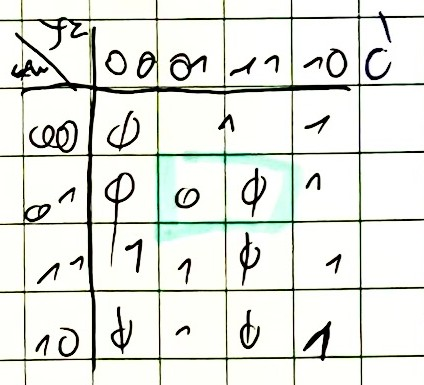
\includegraphics[width=100pt]{images/q5_3c}
				\end{figure}
				ולכן:
				\[ \bm{F_c = (z' + w + x)} \]
				\item נבחין ש־\hfil $\ol{F_{d}} = {\color{gr}zw'x'} + {\color{cyan}zwx} + {\color{red}ywx'}$
				\begin{figure}[H]
					\centering
					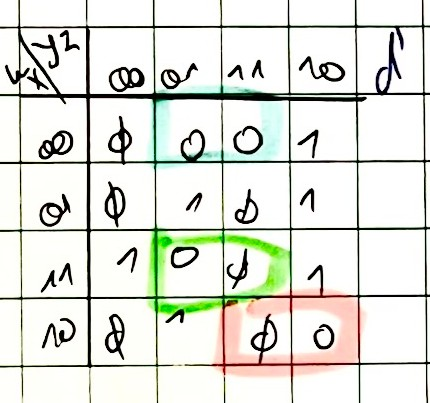
\includegraphics[width=100pt]{images/q5_3d}
				\end{figure}
				ולכן: 
				\[ \bm{F_d = (z' + w + x)(z' + w' + x')(y' + w' + x)} \]
			\end{enumerate}
%		\end{multicols}
		
	\end{enumerate}
	
	
	
	\ndoc
\end{document}